\section{Prior update: Optimal Bayesian Kalman Filter}

\begin{frame}
    \tableofcontents[currentsection]
\end{frame}

\subsection{Basic Idea}
\begin{frame}{Basic Idea: OBKF}
    \begin{itemize}
        \item Based on the IBR Kalman Filter
        \item Utilize measured data $\mathcal{Y}_{k}=\{{\bf y}_0,...,{\bf y}_{k}\}$to obtain the posterior distribution $\pi(\theta|\mathcal{Y}_k)$
        \item Optimize the estimation over the posterior distribution 
    \end{itemize}
\end{frame}


\subsection{Algorithm}
\begin{frame}{Algorithm: OBKF}

OBKF is obtained just replacing ${\bf Q}$ and ${\bf R}$ in Calssic Kalman Filter with $E_{\theta_1}[{\bf Q^{\theta_1}}|\mathcal{Y}_k]$ and $E_{\theta_1}[{\bf R^{\theta_2}}|\mathcal{Y}_k]$ respectively
\begin{algorithm}[H]
\caption{OBKF}
\begin{algorithmic}[1]
\REQUIRE ${\bf \hat x}^{\theta}_k$, $E_\theta[{\bf P^{x, \theta}}_{k}|\mathcal{Y}_{k-1}]$, $\mathcal{Y}_k$
\STATE $\tilde {\bf z}^{\bf \theta}_k = {\bf y}^{\bf \theta}_k - {\bf H}_k{\bf \hat x}^{\bf \theta}_k$
\STATE ${\bf K}^{\bf \Theta^*}_k = E_\theta[{\bf P^{x, \theta}}_k|\mathcal{Y}_{k-1}]{\bf H}^T_kE_\theta^{-1}[{\bf H}_k{\bf P^{x, \theta}}_k{\bf H}^T_k+{\bf R^{\theta_2}}|\mathcal{Y}_{k-1}]$
\STATE $\hat{\bf x}^{\theta}_{k+1} = {\bf \Phi}_k{\bf \hat x}^{\theta}_k+{\bf \Phi}_k{\bf K}^{\bf \Theta}_k{\bf \tilde z}^{\theta}_k$
\STATE $E_\theta[{\bf P^{x, \theta}}_{k+1}|\mathcal{Y}_k] = {\bf \Phi}_k({\bf I}-{\bf K}^{\bf \Theta^*}_k{\bf H}_k)E_\theta[{\bf P^{x, \theta}}_k|\mathcal{Y}_k]{\bf \Phi}^T_k + {\bf \Gamma}_kE_{\theta_1}[{\bf Q^{\theta_1}}|\mathcal{Y}_k]{\bf \Gamma}_k^T$
\ENSURE ${\bf \hat x}^{\theta}_{k+1}$, $E_\theta[{\bf P^{x, \theta}}_{k+1}|\mathcal{Y}_{k}]$
\end{algorithmic}
\end{algorithm}

\pause

How to find the posterior expectations: $E_{\theta_1}[{\bf Q^{\theta_1}}|\mathcal{Y}_k]$ and $E_{\theta_1}[{\bf R^{\theta_2}}|\mathcal{Y}_k]$ ?

\end{frame}

\subsection{Find Posterior Expectations}
\begin{frame}{Find Posterior Expectatoins: $E_{\theta_1}[{\bf Q^{\theta_1}}|\mathcal{Y}_k]$ and $E_{\theta_1}[{\bf R^{\theta_2}}|\mathcal{Y}_k]$}
\begin{itemize}
    \item Approximate $E_{\theta_1}[{\bf Q^{\theta_1}}|\mathcal{Y}_k]$ and $E_{\theta_1}[{\bf R^{\theta_2}}|\mathcal{Y}_k]$ using Metropolis Hastings MCMC
    \item MCMC requires the likelihood function $f(\mathcal{Y}_k|\theta)$
    \item $f(\mathcal{Y}_k|\theta)$ is calculated by:
    \begin{itemize}
        \item Marginalize $f(\mathcal{Y}_k, \mathcal{X}_k|\theta)$ over $\mathcal{X}_k$
        \item Taking advantage of Markov Assumption, $f(\mathcal{Y}_k, \mathcal{X}_k|\theta)$ can be factorized
        \item Using factor-graph, this step can simplify and become easy to understand
    \end{itemize}
\end{itemize}
\end{frame}

\subsection{Performance}

\begin{frame}{Performance: Accuracy}
% Good image will inserted here
\begin{figure}[H]
    \begin{center}
    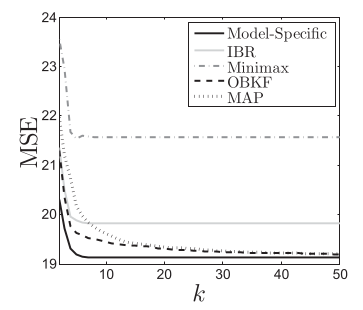
\includegraphics[width=10cm]{img/OBKF_r1.png}
    \caption{Performance analysis for specific $R=\begin{bmatrix} 1 & 1 \\ 1 & 1 \end{bmatrix}$ cited from \cite{Dehghannasiri2018} \protect\linebreak (a) OBKF achieves the lowest MSE \protect\linebreak (b) Empirical average and variance of $E[r|\mathcal{Y}_k]$ }
    \label{fig:r_1}
    \end{center}
\end{figure}
\end{frame}

\begin{frame}{Performance: Data Efficiency}
    
\begin{figure}[H]
    \begin{center}
    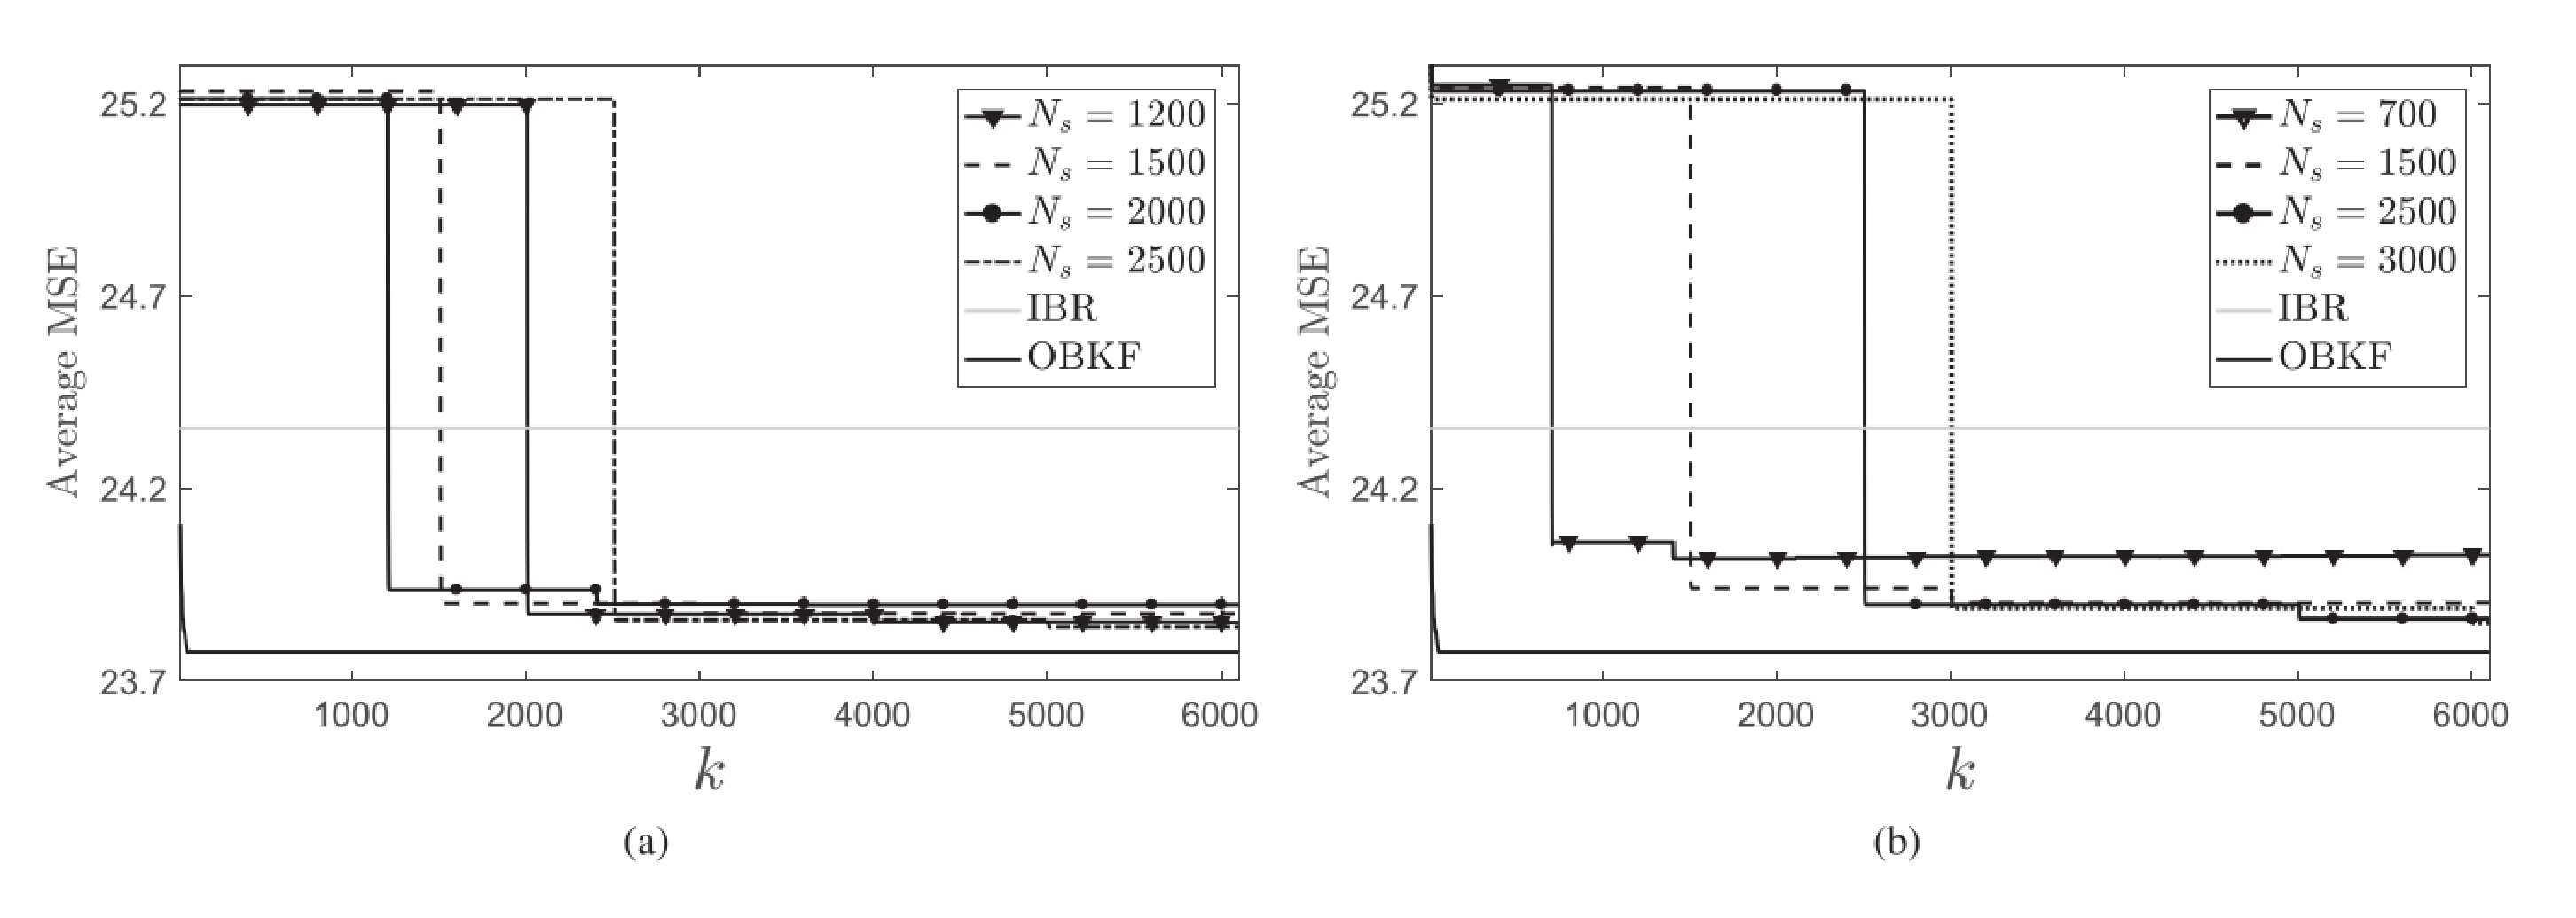
\includegraphics[width=12cm]{img/cmp_adaptive.eps}
    \caption{(a) Unknown r and comparison with the Myers method.\protect\linebreak (b) Unknown r and comparison with the Mehra method. cited from \cite{Dehghannasiri2018}}
    \label{fig:cmp_adaptive}
    \end{center}
\end{figure}

\end{frame}


\subsection{Problems and Future Works}
\begin{frame}{Problems and Future Works}
\begin{itemize}
    \item If the prior distribution doesn't include the true value, the estimation won't converge
    \item Factor-graph and MCMC are computationally expensive. Finding efficient approach is a future work.
\end{itemize}
\end{frame}